\documentclass{article}
\usepackage{tikz}

\begin{document}

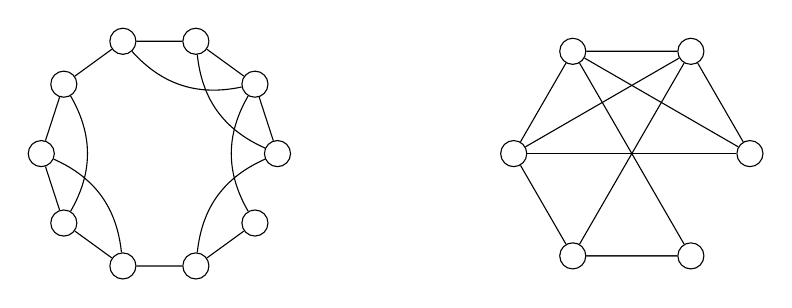
\begin{tikzpicture}[scale=1.5]
    % Define the nodes for the first graph
    \foreach \i in {0,...,9} {
        \node[circle,draw] (A\i) at ({360/10 * \i}:1) {};
    }
    
    % Draw the edges for the first graph
    \draw (A0) -- (A1) -- (A2) -- (A3) -- (A4) -- (A5) -- (A6) -- (A7) -- (A8) -- (A9) -- cycle;
    \draw (A0) to[bend left] (A2);
    \draw (A1) to[bend left] (A3);
    \draw (A4) to[bend left] (A6);
    \draw (A5) to[bend left] (A7);
    \draw (A8) to[bend left] (A0);
    \draw (A9) to[bend left] (A1);

    % Define the nodes for the second graph
    \begin{scope}[xshift=4cm]
        \foreach \i in {0,...,5} {
            \node[circle,draw] (B\i) at ({360/6 * \i}:1) {};
        }
        
        % Draw the edges for the second graph
        \draw (B0) -- (B1) -- (B2) -- (B3) -- (B4) -- (B5) -- cycle;
        \draw (B0) -- (B3);
        \draw (B1) -- (B4);
        \draw (B2) -- (B5);
        \draw (B0) -- (B2);
        \draw (B1) -- (B3);
        \draw (B4) -- (B5);
    \end{scope}
\end{tikzpicture}

\caption{A non $(1,1,4,4)$-packing colorable $1$-saturated graph (on the left) and a non $(1,1,3,3)$-packing colorable $(3,2)$-saturated subcubic graph (on the right).}
\end{document}